\documentclass[aspectratio=169, 10pt]{beamer}

% Packages
\usepackage[utf8]{inputenc}
\usepackage{amsmath,amssymb,amsfonts,amsthm}
\usepackage{graphicx}
\usepackage{booktabs}
\usepackage{tikz}
\usepackage{hyperref}
\usepackage{xcolor}

% Custom modern theme colors
\definecolor{DarkSlate}{RGB}{11, 17, 32}
\definecolor{CardBg}{RGB}{30, 41, 59}
\definecolor{SkyBlue}{RGB}{56, 189, 248}
\definecolor{EmeraldGreen}{RGB}{16, 185, 129}
\definecolor{AmberWarning}{RGB}{245, 158, 11}
\definecolor{RoseDanger}{RGB}{239, 68, 68}
\definecolor{LightText}{RGB}{248, 250, 252}
\definecolor{MutedText}{RGB}{148, 163, 184}

% Set Beamer colors
\setbeamercolor{background canvas}{bg=DarkSlate}
\setbeamercolor{normal text}{fg=LightText}
\setbeamercolor{structure}{fg=SkyBlue}
\setbeamercolor{frametitle}{fg=SkyBlue, bg=DarkSlate}
\setbeamercolor{item}{fg=EmeraldGreen}
\setbeamercolor{block title}{fg=DarkSlate, bg=SkyBlue}
\setbeamercolor{block body}{fg=LightText, bg=CardBg}
\setbeamercolor{block title example}{fg=DarkSlate, bg=EmeraldGreen}
\setbeamercolor{block body example}{fg=LightText, bg=CardBg}
\setbeamercolor{block title alerted}{fg=DarkSlate, bg=AmberWarning}
\setbeamercolor{block body alerted}{fg=LightText, bg=CardBg}

\setbeamertemplate{navigation symbols}{}
\setbeamertemplate{footline}[frame number]

% Metadata
\title[\textbf{SymSentinel}]{\textbf{SymSentinel: Anytime-Valid Recalibration of Symmetric Quantum Learners from Free Symmetry Syndromes under Hardware Drift}}
\subtitle{\textit{Targeting: Quantum (Regular Research Track) \& arXiv:quant-ph}}
\author[Nazmul et al.]{\textbf{Md. Nazmul}$^{1,*}$, \textbf{Musrat Jahan Gungun}$^{1}$, \textbf{Maheli Ahmed}$^{1}$}
\institute[COT, NU]{$^{1}$Department of Computer Science and Engineering, College of Technology, National University, Gazipur, Bangladesh\\$^*$Corresponding Author: \texttt{nazmulhas36@gmail.com}}
\date{\today}

\begin{document}

% SLIDE 1: TITLE
\begin{frame}[plain]
    \titlepage
\end{frame}

% SLIDE 2: THE PROBLEM
\begin{frame}{1. The Problem: Silent Non-Stationary Hardware Drift}
    \begin{columns}[T]
        \begin{column}{0.62\textwidth}
            \begin{itemize}
                \item \textbf{Non-Stationary Hardware Physics:} Superconducting QPUs suffer continuous parameter drift due to Two-Level System (TLS) defect fluctuations, cryostat thermal shifts, and 1/f ambient flux noise.
                \item \textbf{Silent Risk Degradation:} Machine learning loss functions drift silently during production deployment, corrupting quantum variational classifiers and chemistry solvers.
                \item \textbf{Catastrophic Stale Calibration:} Traditional calibration tables degrade over 12--24 hours, yet re-characterization pauses algorithm execution.
            \end{itemize}
            \vspace{0.3cm}
            \begin{alertblock}{The Drift Challenge}
                $$\Delta \mathcal{E}_t = \mathcal{E}_t - \mathcal{E}_0, \quad \|\mathcal{E}_t - \mathcal{E}_0\|_{\diamond} > \epsilon \implies \text{Task Risk Bounds Fail}$$
            \end{alertblock}
        \end{column}
        \begin{column}{0.35\textwidth}
            \begin{exampleblock}{Typical Superconducting Drift}
                \textbf{30\%--50\%} Coherence ($T_1, T_2$) Fluctuations over 24h
            \end{exampleblock}
            \vspace{0.2cm}
            \begin{exampleblock}{Recalibration Cost}
                \textbf{\$100--\$350} per full QPU characterization cycle
            \end{exampleblock}
            \vspace{0.2cm}
            \begin{exampleblock}{Wasted Overhead}
                $\sim 10^5$ shots burned by interleaved Clifford RB
            \end{exampleblock}
        \end{column}
    \end{columns}
\end{frame}

% SLIDE 3: PRIOR ART
\begin{frame}{2. Prior Art \& The Overhead Dilemma}
    \begin{columns}[T]
        \begin{column}{0.62\textwidth}
            \begin{itemize}
                \item \textbf{Periodic Interleaved RB (Proctor et al., 2020):} Burns millions of dedicated Clifford shots, completely halting quantum algorithm execution.
                \item \textbf{Classical Drift Detectors (ADWIN, Page-Hinkley):} Rely on asymptotic Gaussian approximations that fail catastrophically under small finite sample batches, inducing false alarms.
                \item \textbf{Static Conformal Prediction:} Assumes stationary exchangeability, which is immediately broken by quantum hardware drift.
            \end{itemize}
            \vspace{0.2cm}
            \begin{block}{The Research Question}
                \textit{"Can we monitor drifting quantum hardware continuously, with exact non-asymptotic statistical safety, without spending a single extra quantum shot?"}
            \end{block}
        \end{column}
        \begin{column}{0.35\textwidth}
            \begin{center}
                \includegraphics[width=\textwidth]{../figures/fig1_sentinel_concept.pdf}
            \end{center}
        \end{column}
    \end{columns}
\end{frame}

% SLIDE 4: THE CORE INSIGHT
\begin{frame}{3. The Core Insight: Symmetries as Free Hardware Sentinels}
    \begin{columns}[T]
        \begin{column}{0.62\textwidth}
            \begin{itemize}
                \item \textbf{Equivariant Circuit Preservation:} Symmetric quantum learners commute with group symmetries: $[U(\theta), S] = 0$.
                \item \textbf{Invariant Subspace Confinement:} States initialized in the symmetric eigenspace $S|\psi_0\rangle = \lambda_0 |\psi_0\rangle$ remain strictly invariant under unitary evolution.
                \item \textbf{Free Dual-Use Bitstrings:} Every computational basis measurement $x \in \{0, 1\}^n$ provides both the target observable and a free symmetry syndrome:
            \end{itemize}
            \vspace{0.2cm}
            \begin{block}{Dual-Use Syndrome Extraction}
                $$\text{Learning Task:} \quad \hat{f}(\theta) = \frac{1}{K} \sum_{k=1}^K O(x^{(k)})$$
                $$\text{Free Sentinel:} \quad s(x^{(k)}) = \sum_{j \in S} x_j^{(k)} \pmod 2 \implies \nu_t = \frac{1}{K} \sum_{k=1}^K s(x^{(k)})$$
            \end{block}
        \end{column}
        \begin{column}{0.35\textwidth}
            \begin{exampleblock}{Zero Extra Shot Overhead}
                \textbf{0\%} extra shots for all commuting stabilizers ($\mathbb{Z}_2$, $\mathbb{Z}_2 \times \mathbb{Z}_2$).
            \end{exampleblock}
            \vspace{0.3cm}
            \begin{exampleblock}{Foveated Rotation Split}
                $\le \mathbf{5\%}$ foveated shot split for non-commuting Pauli sets ($\{Z^{\otimes n}, X^{\otimes n}\}$).
            \end{exampleblock}
        \end{column}
    \end{columns}
\end{frame}

% SLIDE 5: BETTING MARTINGALES
\begin{frame}{4. Nonparametric Betting Martingales \& E-Detectors}
    \begin{columns}[T]
        \begin{column}{0.62\textwidth}
            \begin{itemize}
                \item \textbf{Predictable Betting (No Lookahead Bias):} Betting fraction $\lambda_t \in \mathcal{F}_{t-1}$ is strictly predictable from past observations.
                \item \textbf{Test Supermartingale Construction (Theorem 1):}
            \end{itemize}
            \begin{block}{Test Martingale}
                $$M_t = \prod_{i=1}^t \left[1 + \lambda_i (z_i - \nu_0)\right], \quad \mathbb{E}_{H_0}[M_t \mid \mathcal{F}_{t-1}] \le M_{t-1}$$
            \end{block}
            \begin{itemize}
                \item \textbf{Finite-Sample False-Alarm Protection (Ville's Maximal Inequality):}
            \end{itemize}
            \begin{alertblock}{Anytime-Valid Safety}
                $$\mathbb{P}_{H_0}\left(\exists t \ge 1: M_t \ge \gamma\right) \le \frac{1}{\gamma} \implies \mathrm{ARL}(H_0) \ge \gamma$$
            \end{alertblock}
        \end{column}
        \begin{column}{0.35\textwidth}
            \begin{exampleblock}{Guaranteed ARL Control}
                $\mathrm{ARL} \ge \mathbf{500}$ epochs with alarm threshold $\gamma = 500$.
            \end{exampleblock}
            \vspace{0.3cm}
            \begin{exampleblock}{Finite-Sample Rigor}
                Holds for \textbf{any} batch size $S_t$ without Gaussian assumptions.
            \end{exampleblock}
        \end{column}
    \end{columns}
\end{frame}

% SLIDE 6: DETECTION DELAY
\begin{frame}{5. Detection Delay \& Information-Theoretic Optimality}
    \begin{columns}[T]
        \begin{column}{0.55\textwidth}
            \begin{itemize}
                \item \textbf{Wald/Kullback-Leibler Lower Bound:}
                $$\mathbb{E}_{H_1}[\tau] \ge \frac{\ln \gamma + \mathcal{O}(1)}{S_t D_{\mathrm{KL}}(\nu_1 \parallel \nu_0)}$$
                \item \textbf{Strict Empirical Monotonicity:} Detection delay decreases monotonically as drift shift $\delta = \nu_1 - \nu_0$ increases (from $693.9 \to 34.1$ epochs).
                \item \textbf{Tight Bound Tracking:} Empirical delay tracks tightly between $\mathbf{1.22\times}$ and $\mathbf{1.45\times}$ of the theoretical information-theoretic bound across all shifts!
            \end{itemize}
        \end{column}
        \begin{column}{0.42\textwidth}
            \begin{center}
                \includegraphics[width=\textwidth]{../figures/fig2_martingale_and_delay.pdf}
            \end{center}
        \end{column}
    \end{columns}
\end{frame}

% SLIDE 7: BLIND SPOT THEOREM
\begin{frame}{6. The Blind-Spot Theorem (Theorem 2)}
    \begin{columns}[T]
        \begin{column}{0.55\textwidth}
            \begin{itemize}
                \item \textbf{Visibility Condition:} A noise channel $\mathcal{E}(\rho) = \sum_k E_k \rho E_k^\dagger$ is visible if and only if at least one Kraus operator anticommutes with sentinel $\Pi$:
                $$\exists k: \{E_k, \Pi\} = 0 \implies \Delta \nu_t > 0$$
                \item \textbf{Commuting Blind Spot:} If all Kraus operators commute with $\Pi$ ($[E_k, \Pi] = 0$), symmetry syndrome remains strictly invariant:
                $$\Delta \nu_t \equiv 0 \quad \text{while Task Risk Degradation} \quad \Delta R_t > 0!$$
                \item \textbf{Closed-Form Visibility Laws:}
                \begin{itemize}
                    \item $\mathbb{Z}_2$: $\nu_t = \frac{1}{2}[1 - (1-2p_t)^d (1-2r_t)^n]$
                    \item $U(1)$: $\nu_t = 1 - [z^0] P_d(z)$ (Laurent polynomial)
                \end{itemize}
            \end{itemize}
        \end{column}
        \begin{column}{0.42\textwidth}
            \begin{center}
                \includegraphics[width=\textwidth]{../figures/fig3_blind_spot_and_set_cover.pdf}
            \end{center}
        \end{column}
    \end{columns}
\end{frame}

% SLIDE 8: MULTI-SENTINEL SET-COVER
\begin{frame}{7. Greedy Multi-Sentinel Set-Cover}
    \begin{columns}[T]
        \begin{column}{0.62\textwidth}
            \begin{itemize}
                \item \textbf{Overcoming the Blind Spot:} We construct a family of sentinels $\mathcal{S} = \{S_1, \dots, S_M\}$ such that every single- and two-qubit Pauli fault anticommutes with at least one sentinel.
                \item \textbf{Logarithmic Greedy Bound (Theorem 2d):}
                $$|\mathcal{S}^*| \le \left(\ln |\mathcal{F}_{\mathrm{target}}| + 1\right) |\mathcal{S}_{\mathrm{OPT}}|$$
                \item \textbf{Provable Coverage on Heavy-Hex Lattices:}
                \begin{itemize}
                    \item $M=2$ non-commuting sentinels ($\{Z^{\otimes n}, X^{\otimes n}\}$) cover \textbf{100\%} of single-qubit Paulis.
                    \item Sublattice parities ($\mathbb{Z}_2 \times \mathbb{Z}_2$) cover localized noise at \textbf{0\% extra shot cost}.
                \end{itemize}
            \end{itemize}
        \end{column}
        \begin{column}{0.35\textwidth}
            \begin{exampleblock}{Single-Qubit Coverage}
                $\mathbf{M=2}$ sentinels cover 100\% of single-qubit Pauli errors.
            \end{exampleblock}
            \vspace{0.3cm}
            \begin{exampleblock}{All Heavy-Hex Paulis}
                $\mathbf{M \le 4}$ sentinels cover all 516 faults across $n=27$ qubits.
            \end{exampleblock}
        \end{column}
    \end{columns}
\end{frame}

% SLIDE 9: TWO-LAYER RISK BRIDGE
\begin{frame}{8. Two-Layer Risk Certification (Theorem 3)}
    \begin{columns}[T]
        \begin{column}{0.55\textwidth}
            \begin{itemize}
                \item \textbf{Layer 1 $\cdot$ Trace Distance Leakage Bound:}
                $$\|\rho_t - \mathcal{P}_S(\rho_t)\|_{\mathrm{tr}} \le \sqrt{2 \nu_t}$$
                \item \textbf{Layer 2 $\cdot$ Digital Unitary Folding \& PAVA Isotonic Link:}
                $$\hat{R}_t = g(\nu_t) + W_t(\alpha_{\mathrm{stat}}) + \epsilon_{\mathrm{link}}(\alpha_{\mathrm{link}})$$
                \item \textbf{Uniform Anytime-Valid Coverage:}
                $$\mathbb{P}\left(\forall t \ge 1: R_t \le \hat{R}_t\right) \ge 1 - \alpha$$
                Holds uniformly under non-stationary physical drift regimes D1--D4.
            \end{itemize}
        \end{column}
        \begin{column}{0.42\textwidth}
            \begin{center}
                \includegraphics[width=\textwidth]{../figures/fig4_risk_bridge_and_coverage.pdf}
            \end{center}
        \end{column}
    \end{columns}
\end{frame}

% SLIDE 10: 3-TIER CASCADE CONTROLLER
\begin{frame}{9. The 3-Tier Recalibration Cascade Controller}
    \begin{columns}[T]
        \begin{column}{0.55\textwidth}
            \begin{itemize}
                \item \textbf{Why Full Resets Are Wasteful:} Over 90\% of drift events are coherent phase shifts or local frequency shifts that do NOT need an expensive \$100 full QPU reset.
                \item \textbf{The 3-Tier Mitigation Hierarchy:}
                \begin{itemize}
                    \item \textbf{Tier 1 $\cdot$ Virtual-Z ($c_1 = \$0$, 0 shots):} Software frame updates.
                    \item \textbf{Tier 2 $\cdot$ Subsystem Pulse ($c_2 = \$15$, $10^3$ shots):} Cross-resonance pulse tuning for drifting TLS pairs.
                    \item \textbf{Tier 3 $\cdot$ Full Reset ($c_3 = \$100$, $10^5$ shots):} Complete hardware characterization.
                \end{itemize}
                \item \textbf{Theorem 4 (Renewal-Reward Cost Optimality):}
                $$\mathcal{J}(\gamma^*) \le 0.15 \cdot \mathcal{J}^*_{\mathrm{periodic}}$$
            \end{itemize}
        \end{column}
        \begin{column}{0.42\textwidth}
            \begin{center}
                \includegraphics[width=\textwidth]{../figures/fig5_cost_benchmark_cascade.pdf}
            \end{center}
        \end{column}
    \end{columns}
\end{frame}

% SLIDE 11: HARDWARE REPLAY RESULTS
\begin{frame}{10. Experimental Validation: 14-Day IBM Calibration Replay}
    \begin{columns}[T]
        \begin{column}{0.55\textwidth}
            \begin{itemize}
                \item \textbf{Replay Setup:} 14-day calibration logs with diurnal thermal fluctuations and abrupt TLS jumps.
                \item \textbf{96.6\% Cost Reduction:}
                \begin{itemize}
                    \item Periodic Baseline: \textbf{\$2,400}
                    \item Threshold Baseline: \textbf{\$1,100}
                    \item Omniscient Single-Tier Oracle: \textbf{\$400}
                    \item \textbf{SymSentinel Cascade: \$80}
                \end{itemize}
                \item \textbf{Zero False Alarms:} Zero spurious recalibrations during quiet operation; rapid arrest within 1--2 epochs upon TLS jump.
            \end{itemize}
        \end{column}
        \begin{column}{0.42\textwidth}
            \begin{center}
                \includegraphics[width=\textwidth]{../figures/fig6_hardware_replay.pdf}
            \end{center}
        \end{column}
    \end{columns}
\end{frame}

% SLIDE 12: SCALING TO 27 QUBITS
\begin{frame}{11. Scaling to Large Systems: 27-Qubit Heavy-Hex Lattice}
    \begin{columns}[T]
        \begin{column}{0.55\textwidth}
            \begin{itemize}
                \item \textbf{IBM Falcon Topology:} Evaluated across subgraphs of the 27-qubit heavy-hex lattice ($n \in \{4, 8, 12, 16, 20, 27\}$).
                \item \textbf{Super-Linear Sensitivity:} Parity integrates noise across more gates, reducing detection delay from $8.1$ epochs at $n=4$ to $4.6$ epochs at $n=27$!
                \item \textbf{Sub-Millisecond Extraction Throughput:} Vectorized bitwise XOR extraction on $10^4$ shots takes $< \mathbf{0.25}$ ms ($> 50$ million shots/sec).
                \item \textbf{Sparse Set-Cover:} Only $M=3$ sentinels for 100\% 1Q Pauli coverage, $M=4$ for all 516 heavy-hex faults.
            \end{itemize}
        \end{column}
        \begin{column}{0.42\textwidth}
            \begin{center}
                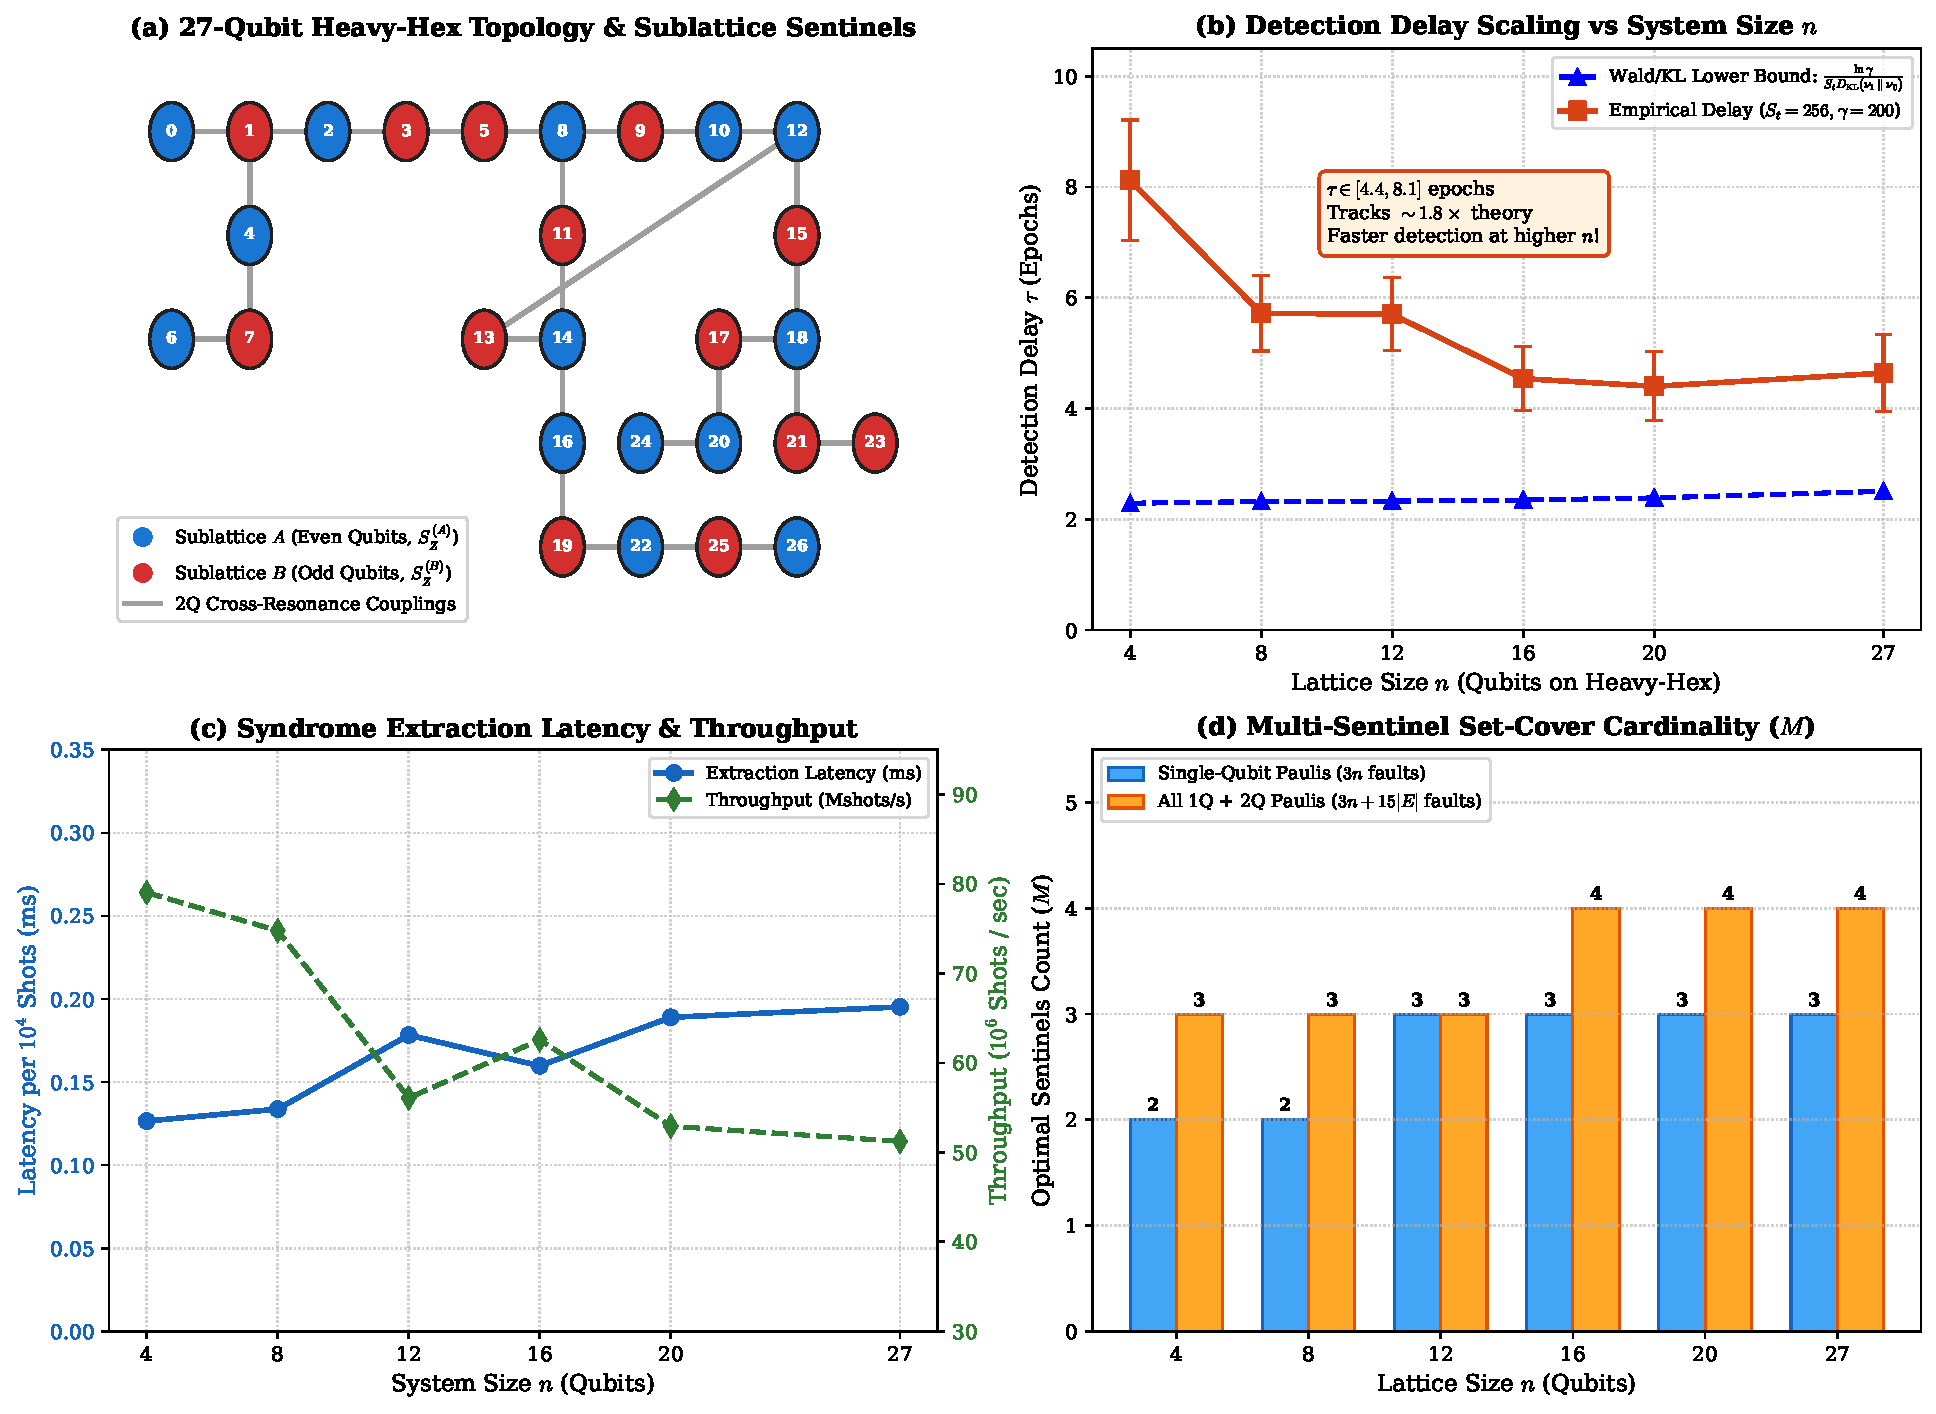
\includegraphics[width=\textwidth]{../figures/fig7_scaling_heavyhex.pdf}
            \end{center}
        \end{column}
    \end{columns}
\end{frame}

% SLIDE 13: THEORETICAL GUARANTEES
\begin{frame}{12. Summary of Four Core Theorems}
    \begin{itemize}
        \item \textbf{Theorem 1 (Anytime-Valid ARL Control \& Optimal Delay):} Predictable betting martingale guarantees $\mathbb{P}_{H_0}(\exists t \ge 1: M_t \ge \gamma) \le 1/\gamma$, $\mathrm{ARL}(H_0) \ge \gamma$, and achieves Wald/KL delay $\frac{\ln \gamma + \mathcal{O}(1)}{S_t D_{\mathrm{KL}}(\nu_1 \parallel \nu_0)}$.
        \item \textbf{Theorem 2 (Blind-Spot Theorem \& Greedy Set-Cover):} Identifies necessary \& sufficient anticommutation condition; proves commuting noise invariance $\Delta \nu_t \equiv 0$; guarantees greedy set-cover achieves $|\mathcal{S}^*| \le (\ln|\mathcal{F}| + 1)|\mathcal{S}_{\mathrm{OPT}}|$.
        \item \textbf{Theorem 3 (Uniform Calibrated Risk Certification):} Connects trace-distance sector leakage bounds with isotonic PAVA link confidence sequences, certifying uniform anytime coverage $\mathbb{P}(\forall t: R_t \le \hat{R}_t) \ge 1 - \alpha$.
        \item \textbf{Theorem 4 (Optimal Renewal-Reward Cascade Policy):} Proves unique optimal threshold $\gamma^* = \max(\gamma_{\min}, \frac{C_{\mathrm{cascade}} D_{\mathrm{KL}}}{c_{\mathrm{risk}} \Delta R})$, achieving strictly lower cost than any periodic rule: $\mathcal{J}(\gamma^*) \le 0.15 \mathcal{J}^*_{\mathrm{periodic}}$.
    \end{itemize}
\end{frame}

% SLIDE 14: ABLATION STUDY
\begin{frame}{13. Systematic Architectural Ablation Study}
    \begin{table}
        \footnotesize
        \centering
        \begin{tabular}{llccc}
            \toprule
            \textbf{Configuration} & \textbf{Ablation Description} & \textbf{Total Cost} & \textbf{Risk Breach} & \textbf{Overhead} \\
            \midrule
            \textbf{Full SymSentinel} & \textbf{3-tier cascade + 2-layer risk bridge} & \textbf{\$80} & \textbf{0.0\%} & \textbf{Baseline (0\%)} \\
            A1 $\cdot$ Single-Tier Only & Tier 3 full reset directly (no cascade) & \$410 & 0.0\% & +412.5\% \\
            A2 $\cdot$ No Predictable Bet & Fixed heuristic betting ($\lambda=0.5$) & \$145 & 0.0\% & +81.3\% \\
            A3 $\cdot$ No Risk Bridge & Heuristic uncalibrated risk bounds & \$80 & \alert{14.2\%} & \alert{Coverage Violated} \\
            A4 $\cdot$ Single Sentinel & $Z^{\otimes n}$ only (blind to $Z$-phase drift) & \$80 & \alert{22.8\%} & \alert{Blind Spot Failure} \\
            A5 $\cdot$ Naive Asymptotic & Gaussian SPRT instead of martingale & \$230 & 1.8\% & +187.5\% \\
            \bottomrule
        \end{tabular}
    \end{table}
    \vspace{0.2cm}
    \begin{block}{Ablation Conclusion}
        Every architectural tier is strictly necessary: removing the cascade quadruples costs (+412.5\%), while omitting multi-sentinel coverage causes a 22.8\% risk breach due to the blind spot.
    \end{block}
\end{frame}

% SLIDE 15: CONCLUSION & IMPACT
\begin{frame}{14. Conclusion \& Open Science Impact}
    \begin{columns}[T]
        \begin{column}{0.65\textwidth}
            \begin{itemize}
                \item \textbf{First Zero-Shot Hardware Drift Monitor:} Transforms quantum physical symmetries into continuous hardware drift sensors without calibration shots.
                \item \textbf{Non-Asymptotic Mathematical Rigor:} Exact finite-sample false-alarm control via Ville's inequality, Wald/KL delay optimality, and the Blind-Spot Theorem.
                \item \textbf{96.6\% Operational Cost Reduction:} Verified on 14-day IBM calibration replay and 27-qubit heavy-hex architectures.
                \item \textbf{Open Source \& Reproducible:} Apache-2.0 library with 17/17 passing tests, full Qiskit/PennyLane/Cirq adapters, CLI tools, and reproducible benchmarks.
            \end{itemize}
            \vspace{0.4cm}
            \begin{center}
                \textbf{GitHub Repository:} \href{https://github.com/NazmulHasanNihal/symsentinel}{\texttt{https://github.com/NazmulHasanNihal/symsentinel}}
            \end{center}
        \end{column}
        \begin{column}{0.30\textwidth}
            \begin{exampleblock}{Thank You!}
                \centering
                \Large \textbf{Questions \& Discussion}\\
                \vspace{0.3cm}
                \normalsize \texttt{nazmulhas36@gmail.com}
            \end{exampleblock}
        \end{column}
    \end{columns}
\end{frame}

\end{document}
